The electronics of the TRITIUM-Aveiro prototype consist of:
\begin{enumerate}
\item{} A PCB designed to power the PMTs with a negative high voltage which consists of several C11152-01  HV power supplies from Hamamatsu Photonics \cite{PowerSupplyAveiroDataSheet}. This PCB is controlled by a MAX5500 DAC\footnote{Digital-to-Analogue Converter} from Maxim Integrated \cite{MAX5500DataSheet}. Its electronic scheme is shown in Figure \ref{fig:ElectronicSchemeHVBoard}.  An Arduino Mega controls the DAC communication and is connected to a Raspberry Pi that runs the whole system. A graphical interface, shown in Figure \ref{fig:GUIHVBoard}, was developed to set up the different options in an easy way.

\begin{figure}[h]
\centering
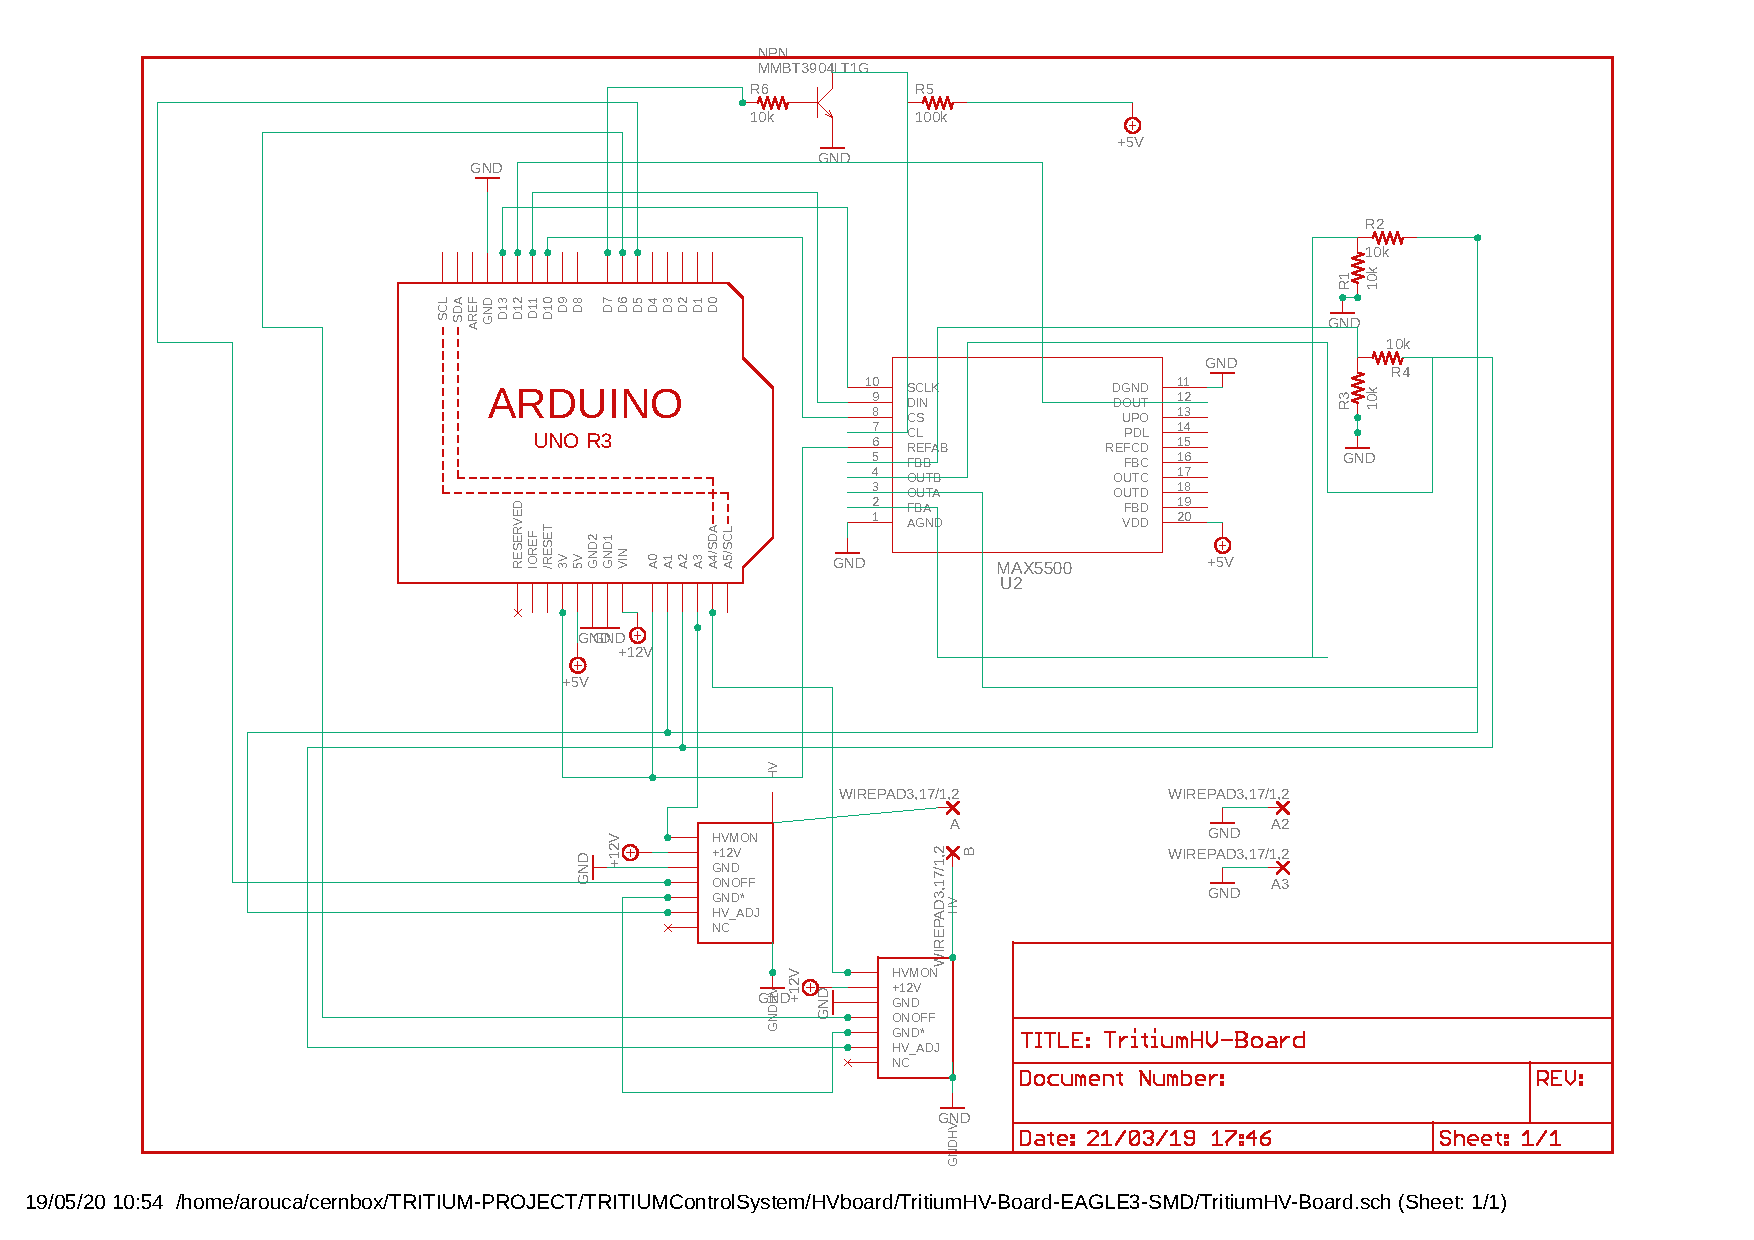
\includegraphics[scale=0.45]{9Appendix/94AveiroElectronics/TritiumHV-Board.pdf}
\caption{Electronic scheme of the PCB designed to power the PMTs of the Aveiro prototype. \label{fig:ElectronicSchemeHVBoard}}
\end{figure}

\begin{figure}[h]
\centering
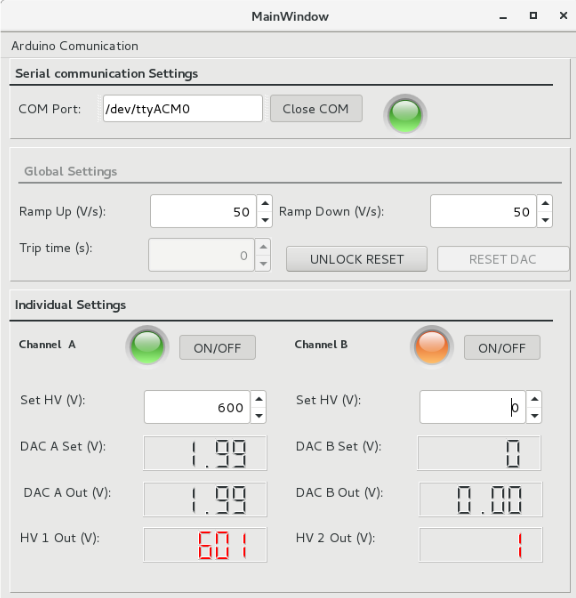
\includegraphics[scale=0.55]{9Appendix/94AveiroElectronics/GUIHVBoard.png}
\caption{Graphical user interface developed to control the prototype. \label{fig:GUIHVBoard}}
\end{figure}

\item{} An electronic chain which consists of several PCBs that process and analyzes the system signals. Its scheme, shown in Figure \ref{fig:ElectronicSchemCounterBoard}, consists of two lines for the PMT signals of the prototype and another one for the active veto PMT.

\begin{figure}[h]
\centering
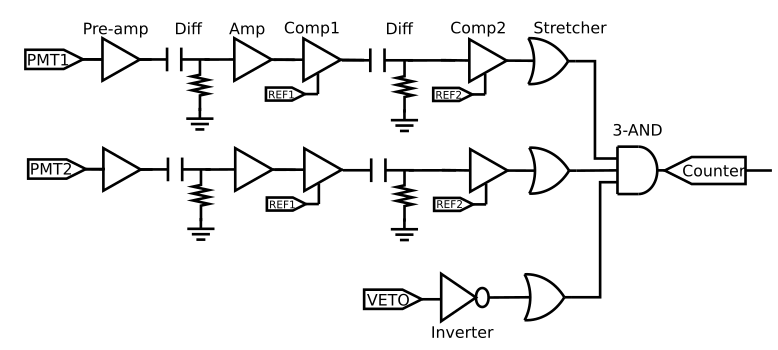
\includegraphics[scale=0.5]{9Appendix/94AveiroElectronics/ElectronicSchemeCounterBoard.png}
\caption{Electronic scheme of the DAQ that process and analyze the signal of the TRITIUM-Aveiro prototype. \label{fig:ElectronicSchemCounterBoard}}
\end{figure}

To test this electronic chain, a plastic scintillator of $10 \times 10 \times 1~\cm^3$ was used as a veto signal. Four different $50\times 30 \times 2~\cm^3$  rectangular vetoes made of plastic scintillator from Saint-Gobain \cite{VetoAveiro} are being built. The vetoes are read out by $2$" R2154-02 PMTs from Hamamatsu Photonics \cite{DataSheetPMTsAveiro}. The PMT signals of the prototype are preamplified and shaped by a CR111 preamplifier from CREMAT Inc. \cite{CREMATPreAmplifierDataSheet}. To reduce electronic noise and signal loss, both preamplifiers are connected as close as possible to the PMTs and they are placed inside aluminium boxes which act as Faraday cages. Each preamplifier is followed by a differentiator stage which reduces the width of the signal and an OPA656 operational amplifier from Texas Instruments \cite{OPA656}. An LT111 fast comparator from Linear Technology \cite{LT111} is used to set a threshold that removes PMT signals with low amplitude (dark counts of the PMTs). A MAX5500 DAC is used to configure the thresholds. As the time width of the amplifier output signal is $200~\mu\second$, a second differentiator was included to reduce random coincidences. To restore a 5V square signal a second comparator was added. Finally, a tunable pulse stretcher based on a SN74AHC1 OR gate from Texas Instruments \cite{Stretcher} sets the signal time width to $100~\nano\second$, obtaining a system coincidence window of $200~\nano\second$.

The veto line consists of an inverter, which gives $0~\volt$ when there is a veto signal and $5~\volt$ otherwise. A stretcher sets the signal time width to $100~\nano\second$.

The signals from the three lines are introduced into a 3-input \\ SN74LVC1G11 AND gate from Texas Instruments \cite{ANDGate} which generates an output signal when both PMT signals are in coincidence and the veto signal is in anti-coincidence. The output signal of this stage is connected to a pulse counter. 

The GPIO pins of a Raspberry Pi are used to communicate with the system and configure the threshold levels. A graphical user interface, shown in Figure \ref{fig:GUIcounts}, was developed to set the counter system in an easy way.
\begin{figure}[h]
\centering
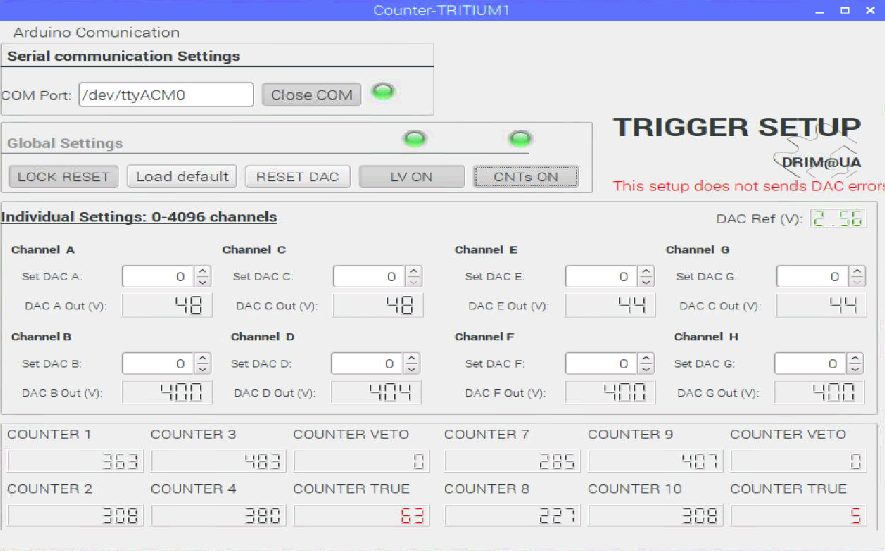
\includegraphics[scale=0.45]{9Appendix/94AveiroElectronics/CounterGUI.png}
\caption{Graphical user interface used to manage the counter system. \label{fig:GUIcounts}}
\end{figure}
In Figure \ref{fig:ScreenshotElectronic}, screenshots for accepted and rejected events are displayed.
\begin{figure}
\centering
    \begin{subfigure}[b]{0.75\textwidth}
    \centering
    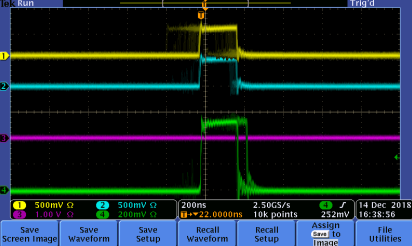
\includegraphics[width=\textwidth]{9Appendix/94AveiroElectronics/Event_accepted_Aveiro_prototype.png}  
    \caption{\label{subfig:TrueTritiumEvent}}
    \end{subfigure}
    \hfill
    \begin{subfigure}[b]{0.75\textwidth}
    \centering
    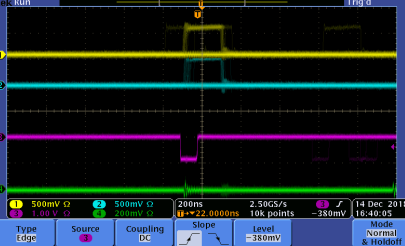
\includegraphics[width=\textwidth]{9Appendix/94AveiroElectronics/Event_rejected_Aveiro_prototype.png}  
    \caption{\label{subfig:FalseTritiumEvent}}
    \end{subfigure}
 \caption{The yellow and blue lines are the prototype PMT signals, the pink line is the veto PMT signal and the green line is the AND logic output. a) Tritium event accepted since the veto is not fired. b) Background event rejected as the veto is fired.}
 \label{fig:ScreenshotElectronic}
\end{figure}

\end{enumerate}